% LTeX: language=fr
% Copyright © 2023, Loïc Grobol <loic.grobol@gmail.com>
% This document is available under the terms of the Creative Commons Attribution 4.0 International License (CC BY 4.0) (https://creativecommons.org/licenses/by/4.0/)

% Settings
\newcommand\myname{L. Grobol}
\newcommand\mylab{MoDyCo, Université Paris Nanterre}
\newcommand\pdftitle{Apprentissage Automatique : Introduction}
\newcommand\mymail{lgrobol@parisnanterre.fr}
\newcommand\titlepagetitle{\pdftitle}
\newcommand\eventname{M2 Plurital}
\newcommand\eventvenue{Nanterre, France}
\newcommand\eventdate{2024-09-24}

\documentclass[
	xcolor={svgnames},
	aspectratio=169,
	french,
]{beamer}
% Colour palettes from [Paul Tol's technical note](https://personal.sron.nl/~pault/data/colourschemes.pdf) v3.1
% Bright scheme
\definecolor{sronbrightblue}{RGB}{68, 119, 170}
\definecolor{sronbrightcyan}{RGB}{102, 204, 238}
\definecolor{sronbrightgreen}{RGB}{34, 136, 51}
\definecolor{sronbrightyellow}{RGB}{204, 187, 68}
\definecolor{sronbrightred}{RGB}{238, 102, 119}
\definecolor{sronbrightpurple}{RGB}{170, 51, 119}
\definecolor{sronbrightgrey}{RGB}{187, 187, 187}

% Divergent colour scheme (fig 19 in Paul Tol's note)
\definecolor{ptolD01}{RGB}{232,236,251}
\definecolor{ptolD02}{RGB}{217,204,227}
\definecolor{ptolD03}{RGB}{209,187,215}
\definecolor{ptolD04}{RGB}{202,172,203}
\definecolor{ptolD05}{RGB}{186,141,180}
\definecolor{ptolD06}{RGB}{174,118,163}
\definecolor{ptolD07}{RGB}{170,111,158}
\definecolor{ptolD08}{RGB}{153,79,136}
\definecolor{ptolD09}{RGB}{136,46,114}
\definecolor{ptolD10}{RGB}{25,101,176}
\definecolor{ptolD11}{RGB}{67,125,191}
\definecolor{ptolD12}{RGB}{82,137,199}
\definecolor{ptolD13}{RGB}{97,149,207}
\definecolor{ptolD14}{RGB}{123,175,222}
\definecolor{ptolD15}{RGB}{78,178,101}
\definecolor{ptolD16}{RGB}{144,201,135}
\definecolor{ptolD17}{RGB}{202,224,171}
\definecolor{ptolD18}{RGB}{247,240,86}
\definecolor{ptolD20}{RGB}{246,193,65}
\definecolor{ptolD22}{RGB}{241,147,45}
\definecolor{ptolD24}{RGB}{232,96,28}
\definecolor{ptolD25}{RGB}{230,85,24}
\definecolor{ptolD26}{RGB}{220,5,12}
\definecolor{ptolD27}{RGB}{165,23,14}
\definecolor{ptolD28}{RGB}{114,25,14}
\definecolor{ptolD29}{RGB}{66,21,10}

\definecolor{sronmutedindigo}{RGB}{51,34,136}

% And my favourite purple
\definecolor{myfavouritepurple}{RGB}{113, 10, 186}
\definecolor{electricindigo}{RGB}{111, 0, 255}
\definecolor{neonpink}{RGB}{255, 68, 204}


\usetheme[
	sectionpage=progressbar,
	subsectionpage=progressbar,
	progressbar=frametitle,
]{metropolis}
	\colorlet{accent}{neonpink}
	\setbeamercolor{frametitle}{
		use=normal text,
		bg=normal text.bg,
		fg=accent,
	}
	\setbeamercolor{alerted text}{fg=accent}
	\setbeamercolor{progress bar}{fg=accent}
	\makeatletter
		\setlength{\metropolis@progressinheadfoot@linewidth}{0.5pt}
	\makeatother

% Left-align description lists
\defbeamertemplate{description item}{align left}{\insertdescriptionitem\hfill}
\setbeamertemplate{description item}[align left]

% Use non-standard fonts
\usepackage{fontspec}
\usefonttheme{professionalfonts}

\directlua{
	luaotfload.add_fallback(
		"myfallback",
		{
			"NotoColorEmoji:mode=harf;",
			"NotoSans:mode=harf;",
			"DejaVuSans:mode=harf;",
		}
	)
}
 
\setsansfont{Fira Sans}[
	BoldFont={* Semibold},
	RawFeature={fallback=myfallback;multiscript=auto;},
]
\setmonofont[Scale=0.9]{Fira Mono}
\newfontfamily\fallbackfont{Deja Vu Sans}
\newfontfamily\emojifont{Noto Color Emoji}[Renderer=HarfBuzz]
\frenchspacing

% Fix missing glyphs in Fira by delegating to polyglossia/babel
\usepackage{newunicodechar}
	\newunicodechar{ }{~}   % U+202F NARROW NO-BREAK SPACE
	\newunicodechar{ }{ }   % U+2009 THIN SPACE

% Notes on left screen
% \usepackage{pgfpages}
% \setbeameroption{show notes on second screen=left}

\usepackage{polyglossia}
	\setmainlanguage{french}
	\setotherlanguage[variant=british]{english}
	\setotherlanguage{breton}

\usepackage{amsfonts,amssymb}
\usepackage{amsmath,amsthm}
\usepackage{mathtools}	% AMS Maths service pack
	\newtagform{brackets}{[}{]}	% Pour des lignes d'équation numérotées entre crochets
	\mathtoolsset{showonlyrefs, showmanualtags, mathic}	% affiche les tags manuels (\tag et \tag*) et corrige le kerning des maths inline dans un bloc italique voir la doc de mathtools
	\usetagform{brackets}	% Utilise le style de tags défini plus haut
\usepackage{lualatex-math}

\usepackage[math-style=french]{unicode-math}
	\setmathfont[Scale=1.3]{Libertinus Math}
\usepackage{newunicodechar}
	\newunicodechar{√}{\sqrt}
\usepackage{mleftright}

% Fix incompatibility with unicode-math
\let\UnicodeMathMathBfSfIt\mathbfsfit
\let\mathbfsfit\relax
\usepackage{mismath}
\let\mathbfsfit\UnicodeMathMathBfSfIt

\usepackage{covington}
\usepackage{tabularx}
\usepackage{booktabs}
\usepackage{siunitx}
	\sisetup{
		detect-all,
		group-separator=\text{\,},
	}
	\DeclareSIUnit{\quantity}{\relax}
	\DeclareSIUnit{\words}{words}
	\DeclareSIUnit{\sentences}{sentences}
	% Needed for italics and bold numbers in siunitx S-aligned columns
	\robustify\itshape
	\robustify\bfseries
\usepackage{multicol}
\usepackage{ccicons}
\usepackage{bookmark}
\usepackage{caption}
	\captionsetup{skip=1ex, labelformat=empty}
\usepackage{lua-ul}
% \usepackage{minted}
% 	\usemintedstyle{lovelace}
% 	\setminted{autogobble, fontsize=\normalsize, tabsize=4}
% 	\setmintedinline{fontsize=auto}
% 	\RenewDocumentCommand\listingscaption{}{Example} 

\usepackage[
	english=american,
	french=guillemets,
	autostyle=true,
]{csquotes}
	\renewcommand{\mkbegdispquote}[2]{\itshape\let\emph\textbf}
	% Like `\foreignquote` but use the outside language's quotes not the inside's
	\NewDocumentCommand\quoteforeign{m m}{\enquote{\textlang{#1}{\textit{#2}}}}

\usepackage{tikz}
	\NewDocumentCommand\textnode{O{}mm}{
		\tikz[remember picture, baseline=(#2.base), inner sep=0pt]{\node[#1] (#2) {#3};}
	}
	\NewDocumentCommand\mathnode{O{}mm}{
		\tikz[remember picture, baseline=(#2.base), inner sep=0pt]{\node[#1] (#2) {\(\displaystyle #3\)};}
	}
	% Beamer utilities
	\tikzset{
		alt/.code args={<#1>#2#3}{%
		  \alt<#1>{\pgfkeysalso{#2}}{\pgfkeysalso{#3}} % \pgfkeysalso doesn't change the path
		},
		invisible/.style={opacity=0},
		visible on/.style={alt={<#1>{}{invisible}}},
		accent on/.style={alt={<#1>{draw=accent, text=accent, thick}{draw}}},
	}
	% Misc utilities
	\tikzset{
		true scale/.style={scale=#1, every node/.style={transform shape}},
	}
	% Custom styles
	\tikzset{
		>=stealth,
		hair lines/.style={line width = 0.05pt, lightgray},
		true scale/.style={scale=#1, every node/.style={transform shape}},
	}	

	\usetikzlibrary{tikzmark}
	\usetikzlibrary{matrix, chains, graphs, graphdrawing}
	\usetikzlibrary{shapes, shapes.geometric}
	\usetikzlibrary{decorations.pathreplacing}
	\usetikzlibrary{decorations.pathmorphing}
	\usetikzlibrary{positioning, calc, intersections}
	\usetikzlibrary{fit}

% % Highlight formulas
% \usepackage[beamer, markings]{hf-tikz}

% \usepackage{forest}
% 	\useforestlibrary{linguistics}

% \usepackage{tikz-dependency}

% Plots
\usepackage{pgfplots}
	\pgfplotsset{compat=1.18}
	% Due to pgfplots meddling with pgfkeys, we have to redefine alt here.
	\pgfplotsset{
		alt/.code args={<#1>#2#3}{%
		\alt<#1>{\pgfkeysalso{#2}}{\pgfkeysalso{#3}} % \pgfkeysalso doesn't change the path
		},
	}
	\pgfplotsset{compat=1.18}
	\pgfplotsset{colormap={SRON}{rgb255=(61,82,161) rgb255=(255,250,210) rgb255=(174,28,62)}} % chktex 36

\usepackage{robust-externalize}

	% \robExtConfigure{
	% 	add to preset={tikz}{
	% 	% we load some packages that will be loaded by figures based on the tikz preset
	% 	add to preamble={\usepackage{pifont}}
	% 	}
	% }

\usepackage[
	block=ragged,
	dashed=false,
	doi=false,
	isbn=false,
	maxbibnames=6,
	maxcitenames=2,
	minbibnames=1,
	mincitenames=1,
	uniquelist=false,
	useprefix=true,
	style=authoryear,
]{biblatex}
	% No small caps in french bib
	\DefineBibliographyExtras{french}{\restorecommand\mkbibnamefamily}
	\AtEveryBibitem{
		\ifentrytype{online}
		{} {
			\iffieldequalstr{howpublished}{online}
			{
				\clearfield{howpublished}
			} {
				\clearfield{urlyear}\clearfield{urlmonth}\clearfield{urlday}
			}
		}
	}
	% Fix bug with \insertbiblabel in author-date, see https://tex.stackexchange.com/questions/585635/beamer-biblatex-authoryear-causes-problem-with-insertbiblabel and https://github.com/josephwright/beamer/blob/865a19d4ec64f4c8e4935c19e162b8f4fd5aa190/base/beamerbaselocalstructure.sty#L501
	\let\insertbiblabel\relax
	\addbibresource{biblio.bib}
 
% Compact bibliography style
\setbeamertemplate{bibliography item}[text]

\AtEveryBibitem{
	\clearfield{series}
	\clearfield{pages}
	\clearname{editor}
}
\renewcommand*{\bibfont}{\tiny}

\usepackage{hyperxmp}	% XMP metadata

\usepackage[type={CC},modifier={by},version={4.0}]{doclicense}

% \usepackage{todonotes}
% 	\let\todox\todo
% 	\renewcommand\todo[1]{\todox[inline]{#1}}

\title{\titlepagetitle}
\author{\textbf{\myname}~(\mylab)}
\institute{}
\date{\eventname\\\eventvenue, \eventdate}

\titlegraphic{\ccby}

% Commands spécifiques
\NewDocumentCommand\shorturl{ O{https} O{://} m }{%
	\href{#1#2#3}{\nolinkurl{#3}}%
}

\DeclarePairedDelimiterX\compset[2]{\lbrace}{\rbrace}{#1\,\delimsize|\,#2}
\DeclarePairedDelimiterX\innprod[2]{\langle}{\rangle}{#1\,\delimsize|\,#2}

% Easy column vectors \vcord{a,b,c} ou \vcord[;]{a;b;c}
% Here be black magic
\ExplSyntaxOn % chktex 1
	\NewDocumentCommand{\vcord}{O{,}m}{\vector_main:nnnn{p}{\\}{#1}{#2}}
	\NewDocumentCommand{\tvcord}{O{,}m}{\vector_main:nnnn{psmall}{\\}{#1}{#2}}
	\seq_new:N\l__vector_arg_seq
	\cs_new_protected:Npn\vector_main:nnnn #1 #2 #3 #4{
		\seq_set_split:Nnn\l__vector_arg_seq{#3}{#4}
		\begin{#1matrix}
			\seq_use:Nnnn\l__vector_arg_seq{#2}{#2}{#2}
		\end{#1matrix}
	}
\ExplSyntaxOff % chktex 1

\NewDocumentCommand\itpause{}{%
	\addtocounter{beamerpauses}{-1}%
	\pause%
}

\NewDocumentCommand\graphdot{O{fill=black} r() O{0.5ex}}{\path[#1] (#2) circle (#3)}


% ██████   ██████   ██████ ██    ██ ███    ███ ███████ ███    ██ ████████
% ██   ██ ██    ██ ██      ██    ██ ████  ████ ██      ████   ██    ██
% ██   ██ ██    ██ ██      ██    ██ ██ ████ ██ █████   ██ ██  ██    ██
% ██   ██ ██    ██ ██      ██    ██ ██  ██  ██ ██      ██  ██ ██    ██
% ██████   ██████   ██████  ██████  ██      ██ ███████ ██   ████    ██

\begin{document}
\pdfbookmark[2]{Title}{title}

\begin{frame}[plain]
	\titlepage
\end{frame}

\begin{frame}<-9>[fragile, plain]
	\begin{center}
		\begin{tikzpicture}[
			focus/.style={draw=ptolD15, thick},
		]
			% Population 1
			\begin{scope}
				\graphdot[fill=ptolD10] (-5.77, 3.89);
				\graphdot[fill=ptolD10] (-5.73, 2.98);
				\graphdot[fill=ptolD10] (-4.27, 2.86);
				\graphdot[fill=ptolD10] (-3.72, 3.86);
				\graphdot[fill=ptolD10] (-5.01, 3.49);
				\graphdot[fill=ptolD10] (-4.74, 2.06);
				\graphdot[fill=ptolD10] (-3.36, 2.10);
				\graphdot[fill=ptolD10] (-2.78, 2.80);
				\graphdot[fill=ptolD10] (-3.76, 3.14);
				\graphdot[fill=ptolD10] (-3.71, 2.58);
				\graphdot[fill=ptolD10] (-5.09, 2.59);
				\graphdot[fill=ptolD10] (-4.46, 1.48);
				\graphdot[fill=ptolD10] (-3.06, 1.79);
				\graphdot[fill=ptolD10] (-4.22, 2.12);
			\end{scope}

			% Population 2
			\begin{scope}
				\graphdot[fill=ptolD26] (2.44, -1.32);
				\graphdot[fill=ptolD26] (2.23, -2.23);
				\graphdot[fill=ptolD26] (2.64, -2.48);
				\graphdot[fill=ptolD26] (3.63, -2.78);
				\graphdot[fill=ptolD26] (4.91, -3.30);
				\graphdot[fill=ptolD26] (5.35, -2.26);
				\graphdot[fill=ptolD26] (4.54, -2.06);
				\graphdot[fill=ptolD26] (4.61, -2.78);
				\graphdot[fill=ptolD26] (4.91, -1.32);
				\graphdot[fill=ptolD26] (3.75, -1.51);
				\graphdot[fill=ptolD26] (3.48, -2.35);
				\graphdot[fill=ptolD26] (4.17, -2.36);
				\graphdot[fill=ptolD26] (3.88, -1.83);
				\graphdot[fill=ptolD26] (2.82, -1.44);
			\end{scope}

			% Extra points 1
			\graphdot[
				fill=black,
				alt={<1,4->{opacity=0}{focus}},
				alt={<3>{fill=ptolD26}{}}
			] (2.0,-1.0);

			\graphdot[
				fill=black,
				alt={<-3, 6->{opacity=0}{focus}},
				alt={<5>{fill=ptolD10}{}}
			] (-2.0,1.0);

			\graphdot[
				fill=black,
				alt={<-5>{opacity=0}{focus}},
				alt={<9>{fill=ptolD26}{}}
			] (2.0,2.5);

			\begin{scope}[visible on={7-}]
				% Extra pop 1
				\begin{scope}
					\graphdot[fill=ptolD10] (-5.38, 3.07);
					\graphdot[fill=ptolD10] (-6.26, 2.62);
					\graphdot[fill=ptolD10] (-5.10, 1.94);
					\graphdot[fill=ptolD10] (-5.31, 1.46);
					\graphdot[fill=ptolD10] (-5.77, 2.12);
					\graphdot[fill=ptolD10] (-4.45, 2.22);
					\graphdot[fill=ptolD10] (-4.34, 1.55);
					\graphdot[fill=ptolD10] (-4.30, 1.06);
					\graphdot[fill=ptolD10] (-3.62, 2.63);
					\graphdot[fill=ptolD10] (-3.71, 3.05);
					\graphdot[fill=ptolD10] (-4.45, 3.39);
					\graphdot[fill=ptolD10] (-5.25, 2.58);
					\graphdot[fill=ptolD10] (-6.45, 1.28);
					\graphdot[fill=ptolD10] (-7.25, 0.80);
					\graphdot[fill=ptolD10] (-6.26, 0.52);
					\graphdot[fill=ptolD10] (-6.07, 1.78);
					\graphdot[fill=ptolD10] (-5.39, 0.72);
					\graphdot[fill=ptolD10] (-4.18, 0.68);
					\graphdot[fill=ptolD10] (-5.78, 1.14);
					\graphdot[fill=ptolD10] (-4.77, 0.50);
					\graphdot[fill=ptolD10] (-4.57, 1.18);
					\graphdot[fill=ptolD10] (-4.67, 2.51);
				\end{scope}

				% Extra pop 2
				\begin{scope}
					\graphdot[fill=ptolD26] (0.78, -1.88);
					\graphdot[fill=ptolD26] (1.36, -3.83);
					\graphdot[fill=ptolD26] (0.71, -3.90);
					\graphdot[fill=ptolD26] (2.55, -3.42);
					\graphdot[fill=ptolD26] (2.78, -3.84);
					\graphdot[fill=ptolD26] (1.82, -2.80);
					\graphdot[fill=ptolD26] (3.42, -3.46);
					\graphdot[fill=ptolD26] (3.20, -2.16);
					\graphdot[fill=ptolD26] (2.76, -1.95);
					\graphdot[fill=ptolD26] (3.19, -2.74);
					\graphdot[fill=ptolD26] (2.18, -2.30);
					\graphdot[fill=ptolD26] (2.56, -2.62);
					\graphdot[fill=ptolD26] (1.60, -1.68);
					\graphdot[fill=ptolD26] (4.21, -3.63);
					\graphdot[fill=ptolD26] (1, -3);
					\graphdot[fill=ptolD26] (2, -4);
				\end{scope}
			\end{scope}

			\begin{scope}[visible on={8-}]
				% Extra pop 1
				\begin{scope}
					\graphdot[fill=ptolD10] (-7.29, -0.72);
					\graphdot[fill=ptolD10] (-5.27, -0.87);
					\graphdot[fill=ptolD10] (-4.17, -1.51);
					\graphdot[fill=ptolD10] (-3.26, -0.61);
					\graphdot[fill=ptolD10] (-2.95, -0.83);
					\graphdot[fill=ptolD10] (-2.20, -2.98);
					\graphdot[fill=ptolD10] (-4.74, -3.10);
					\graphdot[fill=ptolD10] (-3.52, -2.56);
					\graphdot[fill=ptolD10] (-3.42, -2.06);
					\graphdot[fill=ptolD10] (-5.69, -1.80);
					\graphdot[fill=ptolD10] (-6.34, -3.23);
					\graphdot[fill=ptolD10] (-4.66, -3.48);
					\graphdot[fill=ptolD10] (-5.66, -2.30);
					\graphdot[fill=ptolD10] (-6.94, -2.10);
				\end{scope}

				% Extra pop 2
				\begin{scope}
					\graphdot[fill=ptolD26] (2.10, 4.03);
					\graphdot[fill=ptolD26] (3.14, 2.72);
					\graphdot[fill=ptolD26] (4.46, 3.90);
					\graphdot[fill=ptolD26] (5.14, 3.86);
					\graphdot[fill=ptolD26] (6.51, 3.15);
					\graphdot[fill=ptolD26] (7.18, 1.22);
					\graphdot[fill=ptolD26] (5.17, 0.90);
					\graphdot[fill=ptolD26] (6.11, 1.42);
					\graphdot[fill=ptolD26] (5.37, 2.89);
					\graphdot[fill=ptolD26] (4.53, 1.71);
					\graphdot[fill=ptolD26] (6.13, 2.18);
					\graphdot[fill=ptolD26] (4.02, 2.64);
				\end{scope}
			\end{scope}
		\end{tikzpicture}
	\end{center}
\end{frame}

\begin{frame}{Apprendre}
	Dans tout ce qui suit, \textit{\alert{apprendre}} a un sens bien particulier :

	\onslide<2->

	\vfill
	\begin{center}
		\Large\alert{Identifier des régularités dans des données.}
	\end{center}

	\vfill
	\begin{itemize}
		\item<3->[→] Pour mieux les \alert<4-5>{comprendre} ou en générer des similaires\onslide<5->{ : \alert{non-supervisé}}
		\item<4->[→] Pour \alert<4-5>{inférer} les propriétés d'objets inconnus\onslide<6>{ : \alert{supervisé}}
	\end{itemize}
\end{frame}

\begin{frame}{Anthropomorphisme}
	La question de l'apprentissage chez les êtres vivants est encore très ouverte, mais il y a de bonnes raisons de penser que ce qu'on fait en apprentissage automatique n'en est \alert{pas} un modèle raisonnable.

	\pause

	C'est très clair en TAL, où nos modèles n'apprennent ni les mêmes choses ni de la même façon que les locuteurices humain⋅es.

	\pause

	En revanche ça peut fournir des approximations intéressantes des conditions d'\alert{accès aux données}.
\end{frame}

\begin{frame}{Anthropomorphisme}
	On va quand même faire un certain nombre d'\alert{abus de langage} parce que c'est pratique et qu'on y est assez prédisposé⋅es

	\pause

	Mais c'est important de garder dans un coin de son esprit que ce sont effectivement des abus de langage.
\end{frame}
\begin{frame}{🐙}
	Toutefois : en soi, ce qu'on fait ici peut être implémenté par des humain⋅es.

	\pause

	Mais en pratique, on le fait plutôt faire par des \alert{machines} :

	\begin{itemize}[<+->]
		\item Les humain⋅es sont mal équipées pour repérer des \textlang{english}{patterns} dans des \alert{données trop vastes}.
		\item Les humain⋅es et les algorithmes d'apprentissage ont des \alert{biais} inductifs très différents
			\begin{itemize}
				\item[→] Espèrément complémentaires.
			\end{itemize}
	\end{itemize}
\end{frame}

\begin{frame}{En linguistique}
	Non-supervisé :
	\begin{itemize}
		\item \alert{Identifier} des classes de mots ayant des propriétés communes (morpho, syntaxe…)
		\item Formuler des \alert{hypothèses phylogénétiques/typologiques} sur les langues (un peu dangereux)
		\item …
	\end{itemize}
	Supervisé :
	\begin{itemize}
		\item Modéliser des phénomènes linguistiques pour l'\alert{annotation} automatique de corpus.
		\item \alert{Modèles cognitifs} computationnels, modèles de langues (normes)
		\item …
	\end{itemize}
\end{frame}

\begin{frame}{Données}
	Fondamentalement, l'apprentissage automatique, c'est donc une question de \alert{données}.

	\pause

	Les résultats, les applications vont dépendre primairement de la \alert{quantité} de données à laquelle on a accès et de leur \alert{distribution}.

	\pause

	C'est une approximation mathématique qui plaît bien en informatique : on suppose qu'il existe un ensemble de données, on a accès à une partie, un \alert{échantillon} de cet ensemble dont on se sert comme une \alert{approximation} du tout.
\end{frame}

\begin{frame}{Données}
	Évidemment, pour qu'on puisse repérer dans cet échantillon des \alert{régularités} intéressantes, il faut qu'il soit suffisamment couvrant pour que ces régularités soient \alert{observables}.

	\pause

	Une stratégie pour ça, c'est de collecter un échantillon \alert{le plus grand possible} en espérant qu'il va couvrir toute la diversité de données.

	\pause

	C'est \emph{possible}, mais pas forcément idéal en pratique : en linguistique par exemple, le lexique et les constructions ne sont pas uniformément présents, et on court le risque de noyer des points de données \alert{rares mais intéressants}.
\end{frame}

\begin{frame}[plain]
	\begin{figure}
		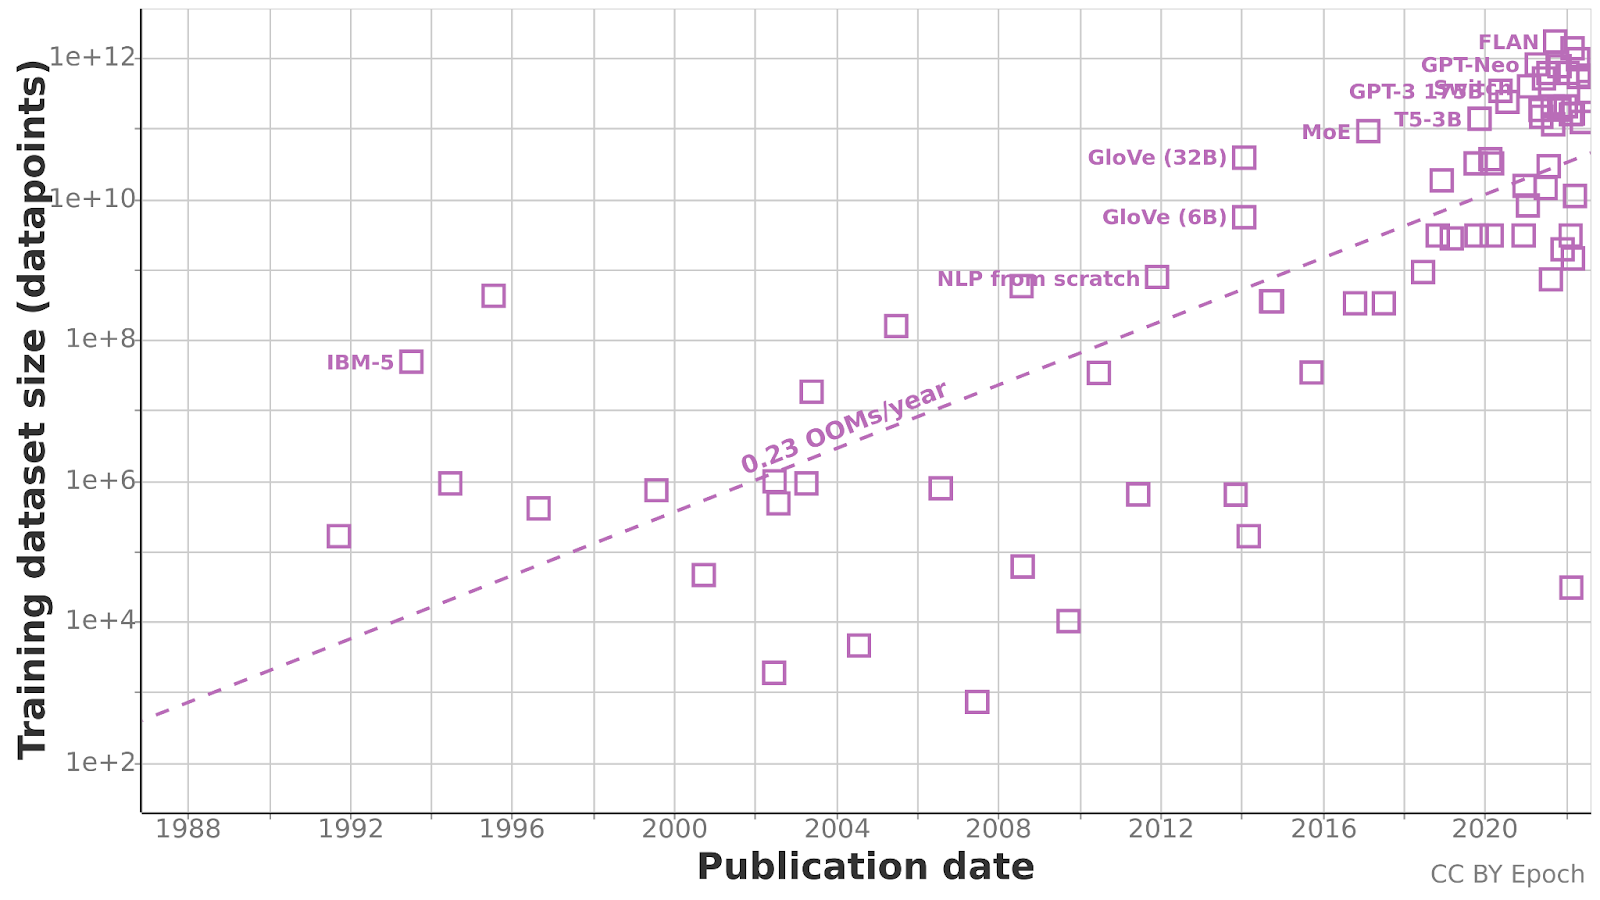
\includegraphics[width=0.9\textwidth]{pics/trends-in-training-dataset-sizes.png}
	\end{figure}
	\parencite{villalobos2022TrendsTrainingDataset}
\end{frame}

\begin{frame}<1>[label=model]{Modèles}
	Même dans le cas les données seraient générées par une règle déterministe, il n'est pas en général possible de la retrouver avec certitude, comme on ne dispose que d'un \alert{échantillon}.

	\pause

	Mais on peut construire différents \alert{modèles} des données avec différentes propriétés.

	\pause

	Le choix d'un modèle est un arbitrage (\quoteforeign{english}{there is no free lunch}) qui dépend des exigences des \alert{applications}.
\end{frame}

\begin{frame}<-4>[fragile, plain]
	\begin{center}
		\begin{tikzpicture}
			% Population 1
			\graphdot[fill=ptolD10] (-5.771476230191826,3.8908509886473874);
			\graphdot[fill=ptolD10] (-5.731442869057548,2.9834281362704065);
			\graphdot[fill=ptolD10] (-4.276897414512093,2.863328052867571);
			\graphdot[fill=ptolD10] (-3.7297748123436194,3.864162081224535);
			\graphdot[fill=ptolD10] (-5.0108423686405335,3.490517377304602);
			\graphdot[fill=ptolD10] (-4.74395329441201,2.0626608301819997);
			\graphdot[fill=ptolD10] (-3.3694745621351125,2.102694191316278);
			\graphdot[fill=ptolD10] (-2.78231859883236,2.809950238021866);
			\graphdot[fill=ptolD10] (-3.769808173477898,3.143561580807521);
			\graphdot[fill=ptolD10] (-3.716430358632193,2.583094524927621);
			\graphdot[fill=ptolD10] (-5.090909090909091,2.596438978639047);
			\graphdot[fill=ptolD10] (-4.46371976647206,1.4888493205906734);
			\graphdot[fill=ptolD10] (-3.06255212677231,1.7957717559534758);
			\graphdot[fill=ptolD10] (-4.223519599666388,2.1293830987391305);

			% Population 2
			\graphdot[fill=ptolD26] (2.4487072560467054,-1.3268304125202521);
			\graphdot[fill=ptolD26] (2.2351959966638866,-2.234253264897233);
			\graphdot[fill=ptolD26] (2.6488740617180984,-2.4877978854143303);
			\graphdot[fill=ptolD26] (3.6363636363636362,-2.7813758670657065);
			\graphdot[fill=ptolD26] (4.91743119266055,-3.301809561811328);
			\graphdot[fill=ptolD26] (5.3577981651376145,-2.2609421723200853);
			\graphdot[fill=ptolD26] (4.543786488740617,-2.0607753666486923);
			\graphdot[fill=ptolD26] (4.610508757297748,-2.7813758670657065);
			\graphdot[fill=ptolD26] (4.91743119266055,-1.3268304125202521);
			\graphdot[fill=ptolD26] (3.756463719766472,-1.5136527644802187);
			\graphdot[fill=ptolD26] (3.489574645537948,-2.3543533483000685);
			\graphdot[fill=ptolD26] (4.170141784820684,-2.3676978020114947);
			\graphdot[fill=ptolD26] (3.8899082568807337,-1.8339196535544473);
			\graphdot[fill=ptolD26] (2.822351959966639,-1.4469304959230878);

			\draw[thick, visible on={2}] (-8, -4.5) -- (8, 4.5);
			\draw[thick, visible on={3}] (0, -4.5) -- (0, 4.5);
			\draw[
				thick,
				decorate,
				decoration={snake, amplitude=3em, segment length=6em},
				visible on={4},
			] (1, -4.5) -- (-1, 4.5);
		\end{tikzpicture}
	\end{center}
\end{frame}

\againframe<1->{model}

\begin{frame}[standout]
	Des idées de propriétés désirables ?
\end{frame}

\begin{frame}{Propriétés des modèles}
	\begin{itemize}[<+->]
		\item Capacités de \alert{mémorisation}.
		\item Capacités d'\alert{extrapolation}.
		\item \alert{Coût} computationnel :
			\begin{itemize}
				\item[→] Pour trouver le modèle.
				\item[→] Pour utiliser le modèle une fois trouvé.
			\end{itemize}
		\item N'importe quelle autre propriété spécifique à l'\alert{application}.
		\item La \alert{simplicité} \onslide<+->{(rasoir d'Occam).}
	\end{itemize}
\end{frame}

\begin{frame}[plain]
	\begin{figure}
        \begin{tikzpicture}[
			data/.style={draw, ellipse},
			program/.style={draw, rectangle},
		]
            \node[data] (in) {Entrée};
            \node[program, color=ptolD10, right=.75cm of in, text width=14ex] (prog) {Programme réalisant la tâche};
            \node[data, right=.75cm of prog] (out) {Résultat};
            \node[program, color=ptolD15, above=1cm of prog, text width=14ex] (progapp) {Programme d'apprentissage};
            \node[data, color=ptolD18, right=.75cm of progapp] (mod) {Modèle};
            \node[data, color=ptolD26, left=.75cm of progapp] (train) {Exemples};
            \draw[->] (in) -- (prog);
            \draw[->] (prog) -- (out);
            \draw[->] (mod) |- ($(prog.north)+(0, 0.5cm)$) -| (prog.north);
            \draw[->] (train) -- (progapp);
            \draw[->] (progapp) -- (mod);
        \end{tikzpicture}
	\end{figure}
\end{frame}

\begin{frame}{Paramètres et hyperparamètres}
	Un modèle généré, \enquote{appris}, par un algorithme d'apprentissage peut être vu comme un ensemble de règles.

	Ces règles (comme tout ce que manipule un ordinateur) sont matérialisées par des valeurs \alert{logiques} ou \alert{numériques} qu'on appelle \alert{paramètres}. Les paramètres d'un modèle sont une représentation (d'une approximation) des données d'entraînement et sont obtenues \emph{a posteriori} dans le processus d'apprentissage.

	\pause

	Les choix \emph{a priori} de l'utilisateurice d'un algorithme d'apprentissage (taille, architecture, variante particulière de l'algorithme, transformations des données…), qui influencent le modèle final, mais ne sont pas \emph{appris}, sont appelés \alert{hyperparamètres}.

	\pause

	Là encore il est très rare qu'on échappe à des arbitrages : \quoteforeign{english}{there is no free lunch}, on ne rase pas gratis.
\end{frame}

\begin{frame}<-3>[label=modelsize]{Taille des modèles}
	Comme pour les données, au-delà de leur expressivité, la \alert{taille} des modèles (en termes de paramètres) est une question omniprésente.

	\pause

	En général : un modèle avec plus de paramètres peut stocker plus d'information, donc \alert{mémoriser} des régularités plus complexes, ce que ne peut pas forcément faire un modèle trop petit (qui \alert{sous-apprendrait}).

	\pause

	Mais un modèle plus gros risque aussi de mémoriser des corrélations fallacieuses ou des biais dans les données au lieu de régularités \alert{intéressantes}. \pause On parle de \alert{sur-apprentissage}.

	\pause

	Débattez de ce dernier mot (3 rounds)
\end{frame}

\begin{frame}[plain]
	\begin{figure}
		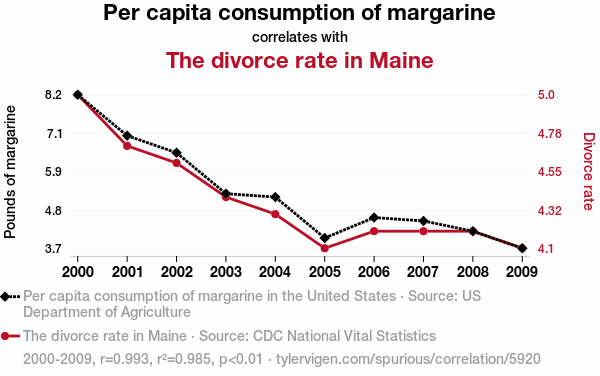
\includegraphics[width=0.9\textwidth]{pics/5920_per-capita-consumption-of-margarine_correlates-with_the-divorce-rate-in-maine.png}
	\end{figure}
	\parencite{vigen2024CapitaConsumptionMargarine}
\end{frame}

\againframe<3->{modelsize}
\begin{frame}[plain]
	\begin{figure}
		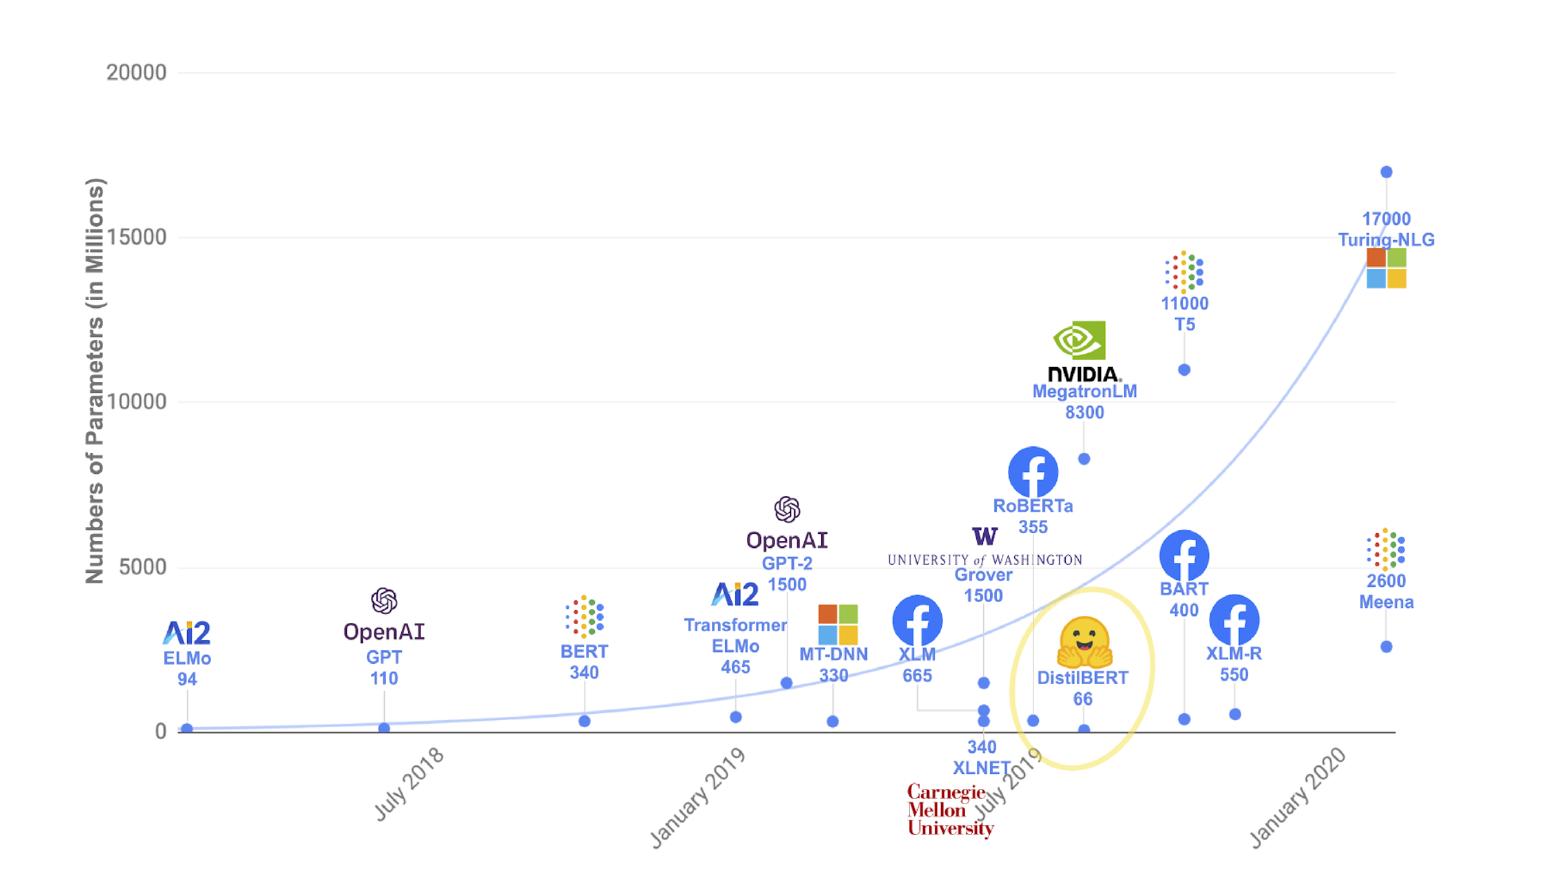
\includegraphics[width=0.9\textwidth]{pics/trends-in-model-sizes.png}
	\end{figure}
	\parencite{mehta2023SemanticTokenizerEnhanced}
\end{frame}

\begin{frame}[plain]
    \vspace{-1\bigskipamount}
    \begin{figure}
        \begin{tikzpicture}
            \begin{axis}[
				xmin=0, xmax=800,
				ymin=0, ymax=600000,
                width=\textwidth,
                height=\textheight,
                % xlabel={Surface},
                % ylabel={Prix},
                title={Population de points},
                % scaled ticks=false,
                % ticklabel style={/pgf/number format/.cd, 1000 sep={\,}},
				xtick=\empty,
				ytick=\empty,
			]
                \addplot[
                    only marks
                ] table [x index=0, y index=1, header=false, row sep=crcr]{
                    150	200000\\
                    155	210000\\
                    160	250000\\
                    170	300000\\
                    200	310000\\
                    260	350000\\
                    300	400000\\
                    600	405000\\
                };
            \end{axis}
        \end{tikzpicture}
    \end{figure}

    {\footnotesize Voir aussi \shorturl{ggbm.at/TagmZdxN}}
\end{frame}

\begin{frame}[plain]
    \vspace{-1\bigskipamount}
    \begin{figure}
        \begin{tikzpicture}
            \begin{axis}[
				xmin=0, xmax=800,
				ymin=0, ymax=600000,
                width=\textwidth,
                height=\textheight,
                % xlabel={Surface},
                % ylabel={Prix},
                title={Régression linéaire : \(y=ax+b\)},
                % scaled ticks=false,
                % ticklabel style={/pgf/number format/.cd, 1000 sep={\,}},
				xtick=\empty,
				ytick=\empty,
			]
                \addplot[
                    only marks
                ] table [x index=0, y index=1, header=false, row sep=crcr]{
                    150	200000\\
                    155	210000\\
                    160	250000\\
                    170	300000\\
                    200	310000\\
                    260	350000\\
                    300	400000\\
                    600	405000\\
                };
                \addplot[ptolD10, domain=0:800, samples=1001] {402.28*x+202807.17};
            \end{axis}
        \end{tikzpicture}
    \end{figure}

	\visible<2>{Léger \alert{sous-apprentissage} (\quoteforeign{english}{underfit})}
\end{frame}

\begin{frame}[plain]
    \vspace{-1\bigskipamount}
    \begin{figure}
        \begin{tikzpicture}
            \begin{axis}[
				xmin=0, xmax=800,
				ymin=0, ymax=600000,
                width=\textwidth,
                height=\textheight,
                % xlabel={Surface},
                % ylabel={Prix},
                title={Régression quadratique : \(y=ax²+bx+c\)},
                % scaled ticks=false,
                % ticklabel style={/pgf/number format/.cd, 1000 sep={\,}},
				xtick=\empty,
				ytick=\empty,
			]
                \addplot[
                    only marks
                ] table [x index=0, y index=1, header=false, row sep=crcr]{
                    150	200000\\
                    155	210000\\
                    160	250000\\
                    170	300000\\
                    200	310000\\
                    260	350000\\
                    300	400000\\
                    600	405000\\
                };
                \addplot[ptolD10, domain=0:800, samples=1001] {-2.56*x^2+2319.29*x-64113.23};
            \end{axis}
        \end{tikzpicture}
    \end{figure}

	\visible<2>{\alert{Sur-apprentissage} (\quoteforeign{english}{overfit})}
\end{frame}

\begin{frame}[plain]
    \vspace{-1\bigskipamount}
    \begin{figure}
        \begin{tikzpicture}
            \begin{axis}[
				xmin=0, xmax=800,
				ymin=0, ymax=600000,
				restrict y to domain=-1000:700000,
				width=\textwidth,
				height=\textheight,
				% xlabel={Surface},
				% ylabel={Prix},
				title={Polynôme d'interpolation de Lagrange : \(y=a₀ + a₁x + a₂x²+ … + a₆x⁶\)},
				% scaled ticks=false,
				% ticklabel style={/pgf/number format/.cd, 1000 sep={\,}},
				xtick=\empty,
				ytick=\empty,
            ]
                \addplot[
                    only marks
                ] table [x index=0, y index=1, header=false, row sep=crcr]{
                    150	200000\\
                    155	210000\\
                    160	250000\\
                    170	300000\\
                    200	310000\\
                    260	350000\\
                    300	400000\\
                    600	405000\\
                };
                \addplot[
					ptolD10,
					domain=100:310,
					samples at={100,101,...,311,311.1,311.15,311.18970915,311.19,311.2,...,312},
				]{
					9.133693238227375E-7*x^6
					-0.0015210072640020665*x^5
					+0.9901617434548338*x^4
					-326.9727250825201*x^3
					+58224.97189714596*x^2
					-5327933.125949258*x
					+196687335.202412
				};
                \addplot[
					ptolD10,
					domain=590:610,
					samples at={
						599.001,599.002,...,599.945,599.9455,599.945526073,599.9456,599.95,599.96,...,600,600.00005,...,610
					},
				]{
					9.133693238227375E-7*x^6
					-0.0015210072640020665*x^5
					+0.9901617434548338*x^4
					-326.9727250825201*x^3
					+58224.97189714596*x^2
					-5327933.125949258*x
					+196687335.202412
				};
            \end{axis}
        \end{tikzpicture}
    \end{figure}

	\visible<2>{\alert{Sur-apprentissage} catastrophique}
\end{frame}

%  █████  ██████  ██████  ███████ ███    ██ ██████  ██ ██   ██
% ██   ██ ██   ██ ██   ██ ██      ████   ██ ██   ██ ██  ██ ██
% ███████ ██████  ██████  █████   ██ ██  ██ ██   ██ ██   ███
% ██   ██ ██      ██      ██      ██  ██ ██ ██   ██ ██  ██ ██
% ██   ██ ██      ██      ███████ ██   ████ ██████  ██ ██   ██

\hypersetup{bookmarksdepth=0}  % Don't create the bookmark for the Appendix part
\appendix
\hypersetup{bookmarksdepth=2}
\bookmarksetup{startatroot}
\section{Appendix}

\pdfbookmark[3]{References}{references}
\begin{frame}[allowframebreaks]{References}
	\printbibliography[heading=none]
\end{frame}

\pdfbookmark[3]{Licence}{licence}
\begin{frame}{Licence}
	\begin{english}
		\begin{center}
			{\huge \ccby}
			\vfill
			This document is distributed under the terms of the Creative Commons Attribution 4.0 International Licence (CC BY 4.0) (\shorturl{creativecommons.org/licenses/by/4.0})

			\vfill
			© 2024, L. Grobol <\shorturl[mailto][:]{loic.grobol@gmail.com}>

			\shorturl[https]{lgrobol.eu}
		\end{center}
	\end{english}
\end{frame}

\end{document}
